\documentclass[letterpaper,12pt]{article}
\setlength{\headheight}{15pt}
\setlength{\marginparwidth}{0pt}
\setlength{\marginparsep}{0pt} % width of space between body text and margin notes
\setlength{\evensidemargin}{0.125in} % Adds 1/8 in. to binding side of all 
% even-numbered pages when the "twoside" printing option is selected
\setlength{\oddsidemargin}{0.125in} % Adds 1/8 in. to the left of all pages when "oneside" printing is selected, and to the left of all odd-numbered pages when "twoside" printing is selected
\setlength{\textwidth}{6.375in} % assuming US letter paper (8.5 in. x 11 in.) and side margins as above
\raggedbottom
\setlength{\parskip}{\medskipamount}


\usepackage{amsmath, amsthm, amssymb, fancyhdr, enumitem, tikz, pgfplots, float}

\pgfplotsset{compat=1.18}

\pagestyle{fancy}
\lhead{CISC684 --- Lecture Notes}
\begin{document}
\section*{Lecture 1}
\paragraph{Supervised Learning}
\paragraph{}Examples are annotated with labels.
\paragraph{Classification}
\paragraph{}Our model will provide labels from a finite set of classes/categories.
\paragraph{CISC684 Notation}
\begin{itemize}
    \item \textbf{Datasets}
\[D = \{\langle x^i, y^i\rangle\,|\, 1 \le i \le N\} \]
$D$ is our dataset, where we have $N$ training instances, and $x^i$ is a training instance, and $y^i$ is a target value.

\item \textbf{Classification}
    \[y^i \in C = \{c_1, \ldots, c_k\}\]
Where $y^i$ is the tartget value for $x^i$. When $k = 2$, we say it is binary classification, and
for $k > 2$, we say it is multi-class classifcation.
\item \textbf{Regression}
\paragraph{}We allow $y^i$ to be a real-valued number in regression.
\end{itemize}
\paragraph{Input Instances}
\paragraph{}Typically our input are specific values for $d$ attributes or features. These values
can be discrete/categorical or numerical. Our input may also be images, or texts, emails, etc.
\paragraph{}Each of our input instances can be represented as vectors of dimension $d$. 
\section*{Lecture 2}
\paragraph{Inductive Bias}
\paragraph{}Strong bias may result in an inability to fit data. The term \textit{high bias} is often used to indicate
the inability to fit training data.
\paragraph{}High bias leads to simple models. We expect simple models to not change
much with small changes to training data (\textit{low variance}).
\paragraph{Noise}
\paragraph{}What is noise?
\begin{itemize}
    \item Errors in labeling data - \textit{teacher noise}
    \item Imprecision in recording the input attributes (shifted data points). 
           \paragraph{} $\langle \ldots, 98.4, \ldots \rangle$
            instead of
            $\langle \ldots, 100.4, \ldots \rangle$
        \item Factors or attributes that are not considered in input representation. (\textit{latent} or
            \textit{hidden} attributes, which are unobserved).
\end{itemize}
\paragraph{Overfitting}
\paragraph{}A stringently trained model may struggle to produce accurate results given noisy data.
\paragraph{Evaluation}
\paragraph{}We may split our dataset into a training set and a test set. The training set being larger,
and the test set being statistically meaningful. 
\paragraph{}The typical split is 90:10, or 80:20.
\paragraph{}During testing time, we predict $y^\prime$ given $x$, and check if $y^\prime = y$.
\paragraph{n-fold Cross-Validation}
\paragraph{} \textbf{Motive:} we may not have a large amount of annotated data.
\paragraph{}In this case, we partition our data into $n$ partitions, and use $n-1$ of these partitions for 
training, and one partition for testing. Then we repeat $n$ times.
\paragraph{}The common practice is 10-fold cross-validation with a training/test split of 90:10.

\paragraph{Learning as Searching}
\paragraph{}Each machine learning method defines a hypothesis space, that is, a certain class of functions
to delineate our data. During training, we search for a "hypothesis" from amongst these functions
which optimizes our model.
\paragraph{Loss Function}
\paragraph{}Loss functions characterize problems a chosen model has in fitting the data. Often
times, loss functions are tied to \textit{error} made by the model on a certain data set. 
\paragraph{}The goal of training is to \textit{minimize} the loss function.
\paragraph{Overfitting with Training}
\paragraph{}With extensive training, overfitting may occur. We may observe this directly if perhaps
validation loss increases as training loss decreases.

\paragraph{Linear Regression}
\paragraph{} \textbf{House Prices:} Can we predice the price of a house based on
\begin{itemize}
    \item $a_1$: Floor area
    \item $a_2$: Number of rooms
    \item $a_3$: Number of bathrooms
    \item $a_4$: Availability of a swimming pool
\end{itemize}
\paragraph{}We assume that house prices may be modeled by some linear function, then we may learn it.
\paragraph{} Let $x^i = \langle a_0, a_1, a_2, a_3, a_4 \rangle$, where $a_0 = 1$. 
\paragraph{}Then our training set $D = 
\{\langle x^1, y^1\rangle\ldots, \langle x^n, y^n \rangle\}$.
\paragraph{}Let $f(x) = w_1x_1 + w_2x_2 +w_3x_3 + w_4x_4 + w_0$.
\paragraph{}Then our model is specified by $w = \langle w_0, w_1, w_2, w_3, w_4 \rangle$.
\paragraph{}And our output vector $O = w \cdot x$
\paragraph{}Let $E(w)$ be the errors on the training set by $w$.
\paragraph{}For a training instance, $x^t$, 
\begin{align*}
    e^t(w) &= y^t - O^t\\
           &= y^t - w \cdot x^t 
\end{align*}
\paragraph{}Then $E(w)$ is simply
\[
    \sum_{i=1}^n (y^t - w \cdot x^t)^2
    \]
\section*{Lecture 3}
\paragraph{Gradient Descent}
\[
    \Delta (w^\prime) = -\eta \frac{\nabla E(w^\prime)}{\nabla w^\prime}
\]
where $0 < \eta < 1$ is the learning rate.
\[
    \to W = w + \Delta w
\]
We use
\[
    W_i = W_i + \Delta w_i
\]
\[
    W_i = - \eta \frac{\partial E(w)}{\partial w_i}
\]
\begin{align*}
    \frac{\partial E(w)}{\partial w_i} &= \frac{\partial}{\partial w_i} \frac{1}{2} \sum_t(y^t-O^t)^2\\
                                       &= \frac{1}{2} \sum_t 2\cdot (y^2-O^t) \cdot \frac{\partial}{\partial w_i}
                                       (y^2 - O^t)\\
                                       &= \sum_t (y^t - O^t)(-x_i^t)
\end{align*}
\begin{align*}
    \to \Delta w_i &= \eta \sum_t(y^t - O^t) x_i^t
\end{align*}
\paragraph{Batching:} Computes gradient descent for partitions or batches of the dataset.
\paragraph{Stochastic Gradient Descent:}
Makes updates based on batch size = 1.

\paragraph{Gradient Descent Algorithm}
\begin{itemize}
    \item Start with a random set of small weights ($w_i$)
    \item While loss is not acceptable:
        \begin{itemize}
            \item Compute loss and gradients
            \item Apply gradients
            \item Recompute model
        \end{itemize}
\end{itemize}

\paragraph{Batching vs. Stochastic}
\paragraph{}Stochastic Gradient Descent can approximate batching with an arbitrary small error.
\paragraph{}SGM can also better avoid local minimas by updating $w$ more frequently. It is also
faster to train, deals with dynamic datasets, and learning rate is usually smaller in SGM.
\paragraph{}Batch training is typically more stable, and easier to check for convergence.
\section*{Lecture 4}
\paragraph{Logistic Regression}
\begin{center}
    
\[
    \mathrm{P}(Y=1\, |\, \hat{x}, \hat{w})
\]
The probability that $\hat{x}$ is a positive instance.

\end{center}

\[
    \sigma(z) = \frac{1}{1+e^{-z}}
\]
\begin{figure}
    \caption{Sigmoid Function}
    \centering
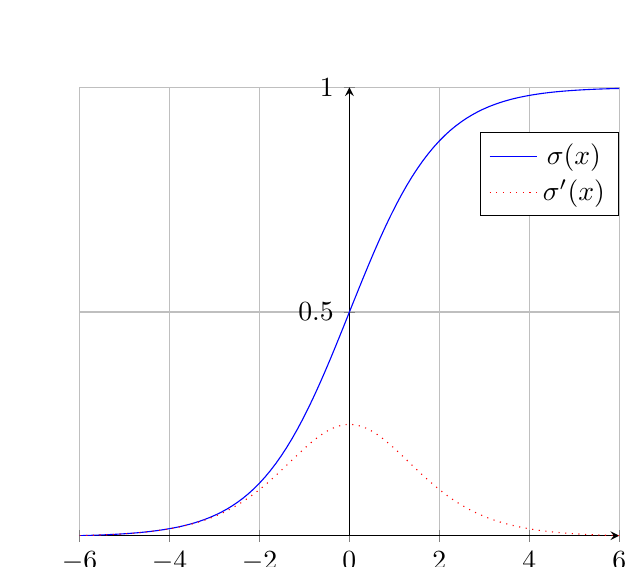
\begin{tikzpicture}[declare function={sigma(\x)=1/(1+exp(-\x));
sigmap(\x)=sigma(\x)*(1-sigma(\x));}]
    
\begin{axis}%
[
    grid=major,     
    xmin=-6,
    xmax=6,
    axis x line=bottom,
    ytick={0,.5,1},
    ymax=1,
    axis y line=middle,
    samples=100,
    domain=-6:6,
    legend style={at={(1,0.9)}}     
]
    \addplot[blue,mark=none]   (x,{sigma(x)});
    \addplot[red,dotted,mark=none]   (x,{sigmap(x)});
    \legend{$\sigma(x)$,$\sigma'(x)$}
\end{axis}
\end{tikzpicture}
\end{figure}

\paragraph{}The sigmoid function will squash our linear output $\to [0,1]$
\[ \mathrm{Output} = \begin{cases}
    1 & P(y=1 \, | \, \hat{x}, \hat{w}) = \sigma(\hat{w}\cdot \hat{x}) \ge 0.5 \\
    0 & \mathrm{else}
    \end{cases}
\]

\paragraph{Maximum Likelihood Estimation:} MLE finds the parameter values that maximize the likelihood
of making the observations given the parameters.
\paragraph{}For a model $\theta$, what is the likelihood of the observed data (training data).

\paragraph{}Given $n$ training instances given by $x^1, x^2, \ldots, x^n$, a model given by parameters $w$, and labels
$y^1, y^2, \ldots, y^n$, the likelihood of the training data is given by

\[
    \mathrm{P}(y^1, y^2, \ldots, y^n \, | \, w, x^2, x^2, \ldots, x^n)
\]
\paragraph{}These instances are independent, thus
\begin{align*}
    \mathrm{P}(y^1, y^2, \ldots, y^n \, | \, w, x^1, x^2, \ldots, x^n)&=
    \mathrm{P}(y^1 \, | \, w, x^1) \cdot \ldots \cdot \mathrm{P}(y^n \, | \, w, x^n) \\
                                                                      &= \prod_{0\le i \le n} 
                                                                      \mathrm{P}(y^i \, | w, x^i)
\end{align*}
\paragraph{}$\prod_t \mathrm{P}(y^t \, | \, w, x^t)$ can be extremely small, leading to underflow problems, so
we take the log and maximize.

\[
    \sum_t \log( \mathrm{P}(y^t \, | \, w, x^t))
\]
\paragraph{}Since $y^t$ is either 0 or 1, we can write this as
\[
    \sum_t y^t\log(\mathrm{P}(y=1 \, | \, w, x^t)) + (1-y^t)\log(\mathrm{P}(y=0 \, | \, w, x^t))
\]
\paragraph{}We use gradient descent to find the $w$ that maximizes this.
\paragraph{Wald Statistic}
\paragraph{}The \textbf{Wald test} is a method for testing whether \textbf{explanatory variables} in a 
model is \textbf{significant}.
\paragraph{}\textbf{"Significant"} indicating that the variable adds to the model. Variables
which do not add anything to the model can be deleted without affecting the model in any meaningful
way.
\paragraph{Logits}
\paragraph{}Rather than converting regression to probability, in statistics, a link function maps
probability to regression.
\paragraph{} \textbf{Logit} is the log of oddds.
\begin{itemize}
    \item $F(x)$ is the probability of success.
    \item Probability of failure is $1-F(x)$.
    \item Odds are defined as $\frac{F(x)}{1-F(x)}$
\end{itemize}

\paragraph{}$F(x) \to [0,1]$, odds thus range between 0 and $\infty$. As $p \to 1$, odds tend
towards infinity.
\begin{table}[htpb]
    \centering
    \begin{tabular}{l r}
    $\displaystyle\lim_{p \to 1}\log(\frac{p}{1-p}) = \infty$, &      
    $\displaystyle\lim_{p \to 0}\log(\frac{p}{1-p}) = -\infty$ 
    \end{tabular}
\end{table}
\section*{Lecture 5}
\subsection*{Decision Trees}
\begin{figure}[H]
    \caption{Example Decision Tree}
    \centering
    \includegraphics[scale=1]{images/dectree.pdf}
\end{figure}
\begin{table}[H]
    \centering
    \caption{Example Dataset}
    \vspace{5mm}
    \begin{tabular}{| c | c | c |}
        \hline
        $A$ & $B$ & Target \\
        \hline
        $a_1$ & $b_1$ & 0 \\
        $a_2$ & $b_2$ & 1 \\
        $a_1$ & $b_2$ & 1 \\
        $a_2$ & $b_1$ & 0  \\
        \hline
    \end{tabular}
\end{table}
\paragraph{}We begin building a decision tree by considering an attribute $A$, $B$, etc. We
consider the values which $A$ may take, $a_1, a_2$. The leaf nodes of our
decision tree \textbf{must be decisions}.

\paragraph{}If we cannot make a decision based on the attributes we have considered, we consider
a new attribute.

\subsection*{Uncertainty}
\paragraph{}Suppose we have attributes $A_1$, $A_2$. $A_1$ has three values:
\begin{table}[H]
    \centering
    \begin{tabular}{c c}
        $c_1$ & 4+/2-\\
        $c_2$ & 2+/2-\\
        $c_3$ & 2+/4-\\
    \end{tabular}
\end{table}
\paragraph{}and $A_2$ has values:
\begin{table}[H]
    \centering
    \begin{tabular}{c c}
        $d_1$ & 5+5-\\
        $d_2$ & 2+/1-\\
        $d_3$ & 1+/2-\\
    \end{tabular}
\end{table}
\paragraph{}Which attribute do we prefer to begin with? \textbf{The attribute which we observe
has less uncertainty.} $A_2$ has a concentration of outcomes on $d_1$ which are evenly stacked,
leading to the overall attribute holding significant uncertainty.
\subsection*{Entropy}
\paragraph{}Let $x$ be a random variable with outcomes $\{a,b,c,d\}$. How many "yes-no" questions
do you need to ask to know the outcome of $x$?

\paragraph{}Suppose
\[
    P(x=a) = \frac{1}{2}, P(x=b) = \frac{1}{4}, P(x=c)=P(x=d)= \frac{1}{8}
\]
\paragraph{}and we form the following tree:
\begin{figure}[H]
    \centering
    \includegraphics[scale=1]{images/entropy.pdf}
\end{figure}
\paragraph{}The expected number of questions we ask is
\[
    \frac{1}{2}\cdot1 + \frac{1}{4}\cdot2 + \frac{1}{8}\cdot3 + \frac{1}{8}\cdot3 = 1.75
\]
\paragraph{}We want to minimize our expected number with an optimal line of inquiry. We can
do this by \textbf{balancing our tree in terms of probability}
\begin{table}[H]
    \centering
    \begin{tabular}{| c | c | c | c |}
        \hline
        $i$ & $P_i$ & $i$ & $f(P_i)$\\
        \hline
        1 & $\frac{1}{2}$ & 1 & $\log_2 \frac{1}{P_i}$\\
        2 & $\frac{1}{4}$ & 2 & $\vdots$\\
        3 & $\frac{1}{8}$ & 3 & $\vdots$\\
        4 & $\frac{1}{8}$ & 3 & $\vdots$\\
        \hline
    \end{tabular}
\end{table}
\paragraph{}We define entropy,
\begin{align*}
    H(x) &= \sum_i P_i \log_2 \frac{1}{P_i}\\
         &= -\sum_i P_i \log_2 \frac{1}{P_i},\\
\end{align*}
\[
    0 \le H(x) \le \log_2(N),
\]
\paragraph{}as our measure of uncertainty.
\paragraph{(Joint entropy, conditional entropy in lecture slides)}

\end{document}



